\lhead{\emph{Introduction}}
\section*{Introduction}
Dans le cadre de la validation de mon diplôme de Master II MIAGE Agilité des Systèmes d'informations à l'université Paris Ouest Nanterre la Défense, on devait effectué un stage de cinq à six mois en entreprise. Ce stage doit permettre de mettre en application les connaissances théoriques et pratiques que j'ai pu acquérir tout au long de ma formation à l'université.
Pour cela j'ai effectué mon stage au site d'ERDF de Mérignac, le stage avait pour thème \og la mise en place d'un outil de travail collaboratif \fg{}. Alors, ce rapport a pour but de présenter le travail que j'ai pu réaliser durant ce stage, il est est composé de quatre parties: 
\begin{itemize}
\item La première partie porte sur la présentation de l'entreprise d'accueil,
\item La seconde partie consiste à présenter le projet avec les objectifs attendus,
\item La troisième partie fait le bilan de ce que j'ai pu réaliser par rapport aux objectifs attendus et aussi les méthodes et techniques employées pour y arriver
\item Et pour finir, nous allons conclure et proposer des perspectives d'amélioration de l'outil.
\end{itemize}
\chapter{Présentation de l'entreprise} % Main chapter title

\label{Chapter1} % Change X to a consecutive number; for referencing this chapter elsewhere, use \ref{ChapterX}

\lhead{Chapitre 1. \emph{Présentation de l'entreprise}} % Change X to a consecutive number; this is for the header on each page - perhaps a shortened title
\section{Historique}
Deux sociétés distinctes ERDF (Électricité Réseau Distribution France) et GRDF (Gaz Réseau Distribution
France) ont été créées le 1er janvier 2008 suite à la scission des activités d'EDF (Électricité De
France) et GDF (Gaz De France).
ERDF, société anonyme et autonome, filiale à 100\% du groupe EDF, est constituée d'un conseil de
surveillance, présidé par Christian Nadal et d'un directoire, présidé par Philippe Mouloubou.
Cette filiale est le gestionnaire de 95\% de réseaux publics de distribution d'électricité.\\
En France, le réseau public de distribution d'électricité appartient aux communes, et aux
regroupements de communes. Celles-ci délèguent l'exploitation, l'entretien et le développement du
réseau présent sur la zone de desserte à ERDF.\\
Partenariat de proximité et innovant, ERDF développe et exploite les réseaux dans le respect de l'environnement et contribue à divers projets de développement social. Sa politique de développement durable associe toutes les parties prenantes (collaborateurs, clients, pouvoir publics, etc).\\
Mission de service public, ERDF assure la continuité et la qualité de la desserte ainsi que l'accès non discriminatoire au réseau public de distribution quelque soit le fournisseur d'électricité. La distribution d'électricité est une activité régulée, contrôlée par la Commission de Régulation de l'Énergie (CRE).
\section{Chiffres clés 2014}
\begin{itemize}
\item ERDF a réalisé un chiffre d'affaires de 13.8 millions d'euros, soit une augmentation de 3.7\% par rapport à 2012.
\item ERDF dispose de 38667 salariés et de 2325 alternants dont 56\% ont été recrutés à la suite de leur période d'apprentissage.
\item ERDF dessert environ 35 millions de clients, a réalisé 11 millions d'interventions et raccordés 436 000 nouveau clients.
\item 1 324 045 km de longueur de réseau Basse Tension (BT) et Moyenne Tension (HTA)
\item 2243 postes sources HTB/HTA
\item 763 812 postes de transformation HTA/BT.
\end{itemize}
\section{Organisation Géographique}
L'implantation d'ERDF en région est assurée, via des Directions Inter Régionales (DIR).
Elles sont au nombre de 8, parmi elles: la DIRSO (Direction Inter Régionale Sud-Ouest) qui possède plusieurs unités opérationnelles:
\begin{itemize}
\item Les Unités Réseau Gaz (URG), chargées de la gestion du réseau Gaz Naturel.
\item Les Unités Clients Fournisseurs (UCF), chargées de l'ensemble des interventions auprès de la clientèle en électricité et en gaz naturel (Mise en Service, Relève des compteurs, etc) et de la
relation clientèle en général.
\item Les Unités Services et Logistique (USL), support des autres unités, dans le domaine de la logistique et des fonctions transverses.
\end{itemize} 
La DIR Sud Ouest, présidée par Gilles CAPY, est constituée de 4 Directions Régionales (DR) et d'une Direction Inter Régionale.
\clearpage
\subsection*{Directions Régionales}
Les DR sont composées de l'état major, service des ressources humaines, service logistique, la direction client et de la Direction Technique.
Elles disposent d'un Directeur Régional et sont situées de la façon suivante~\ref{dirso} : 
\begin{figure}[h]
\centering
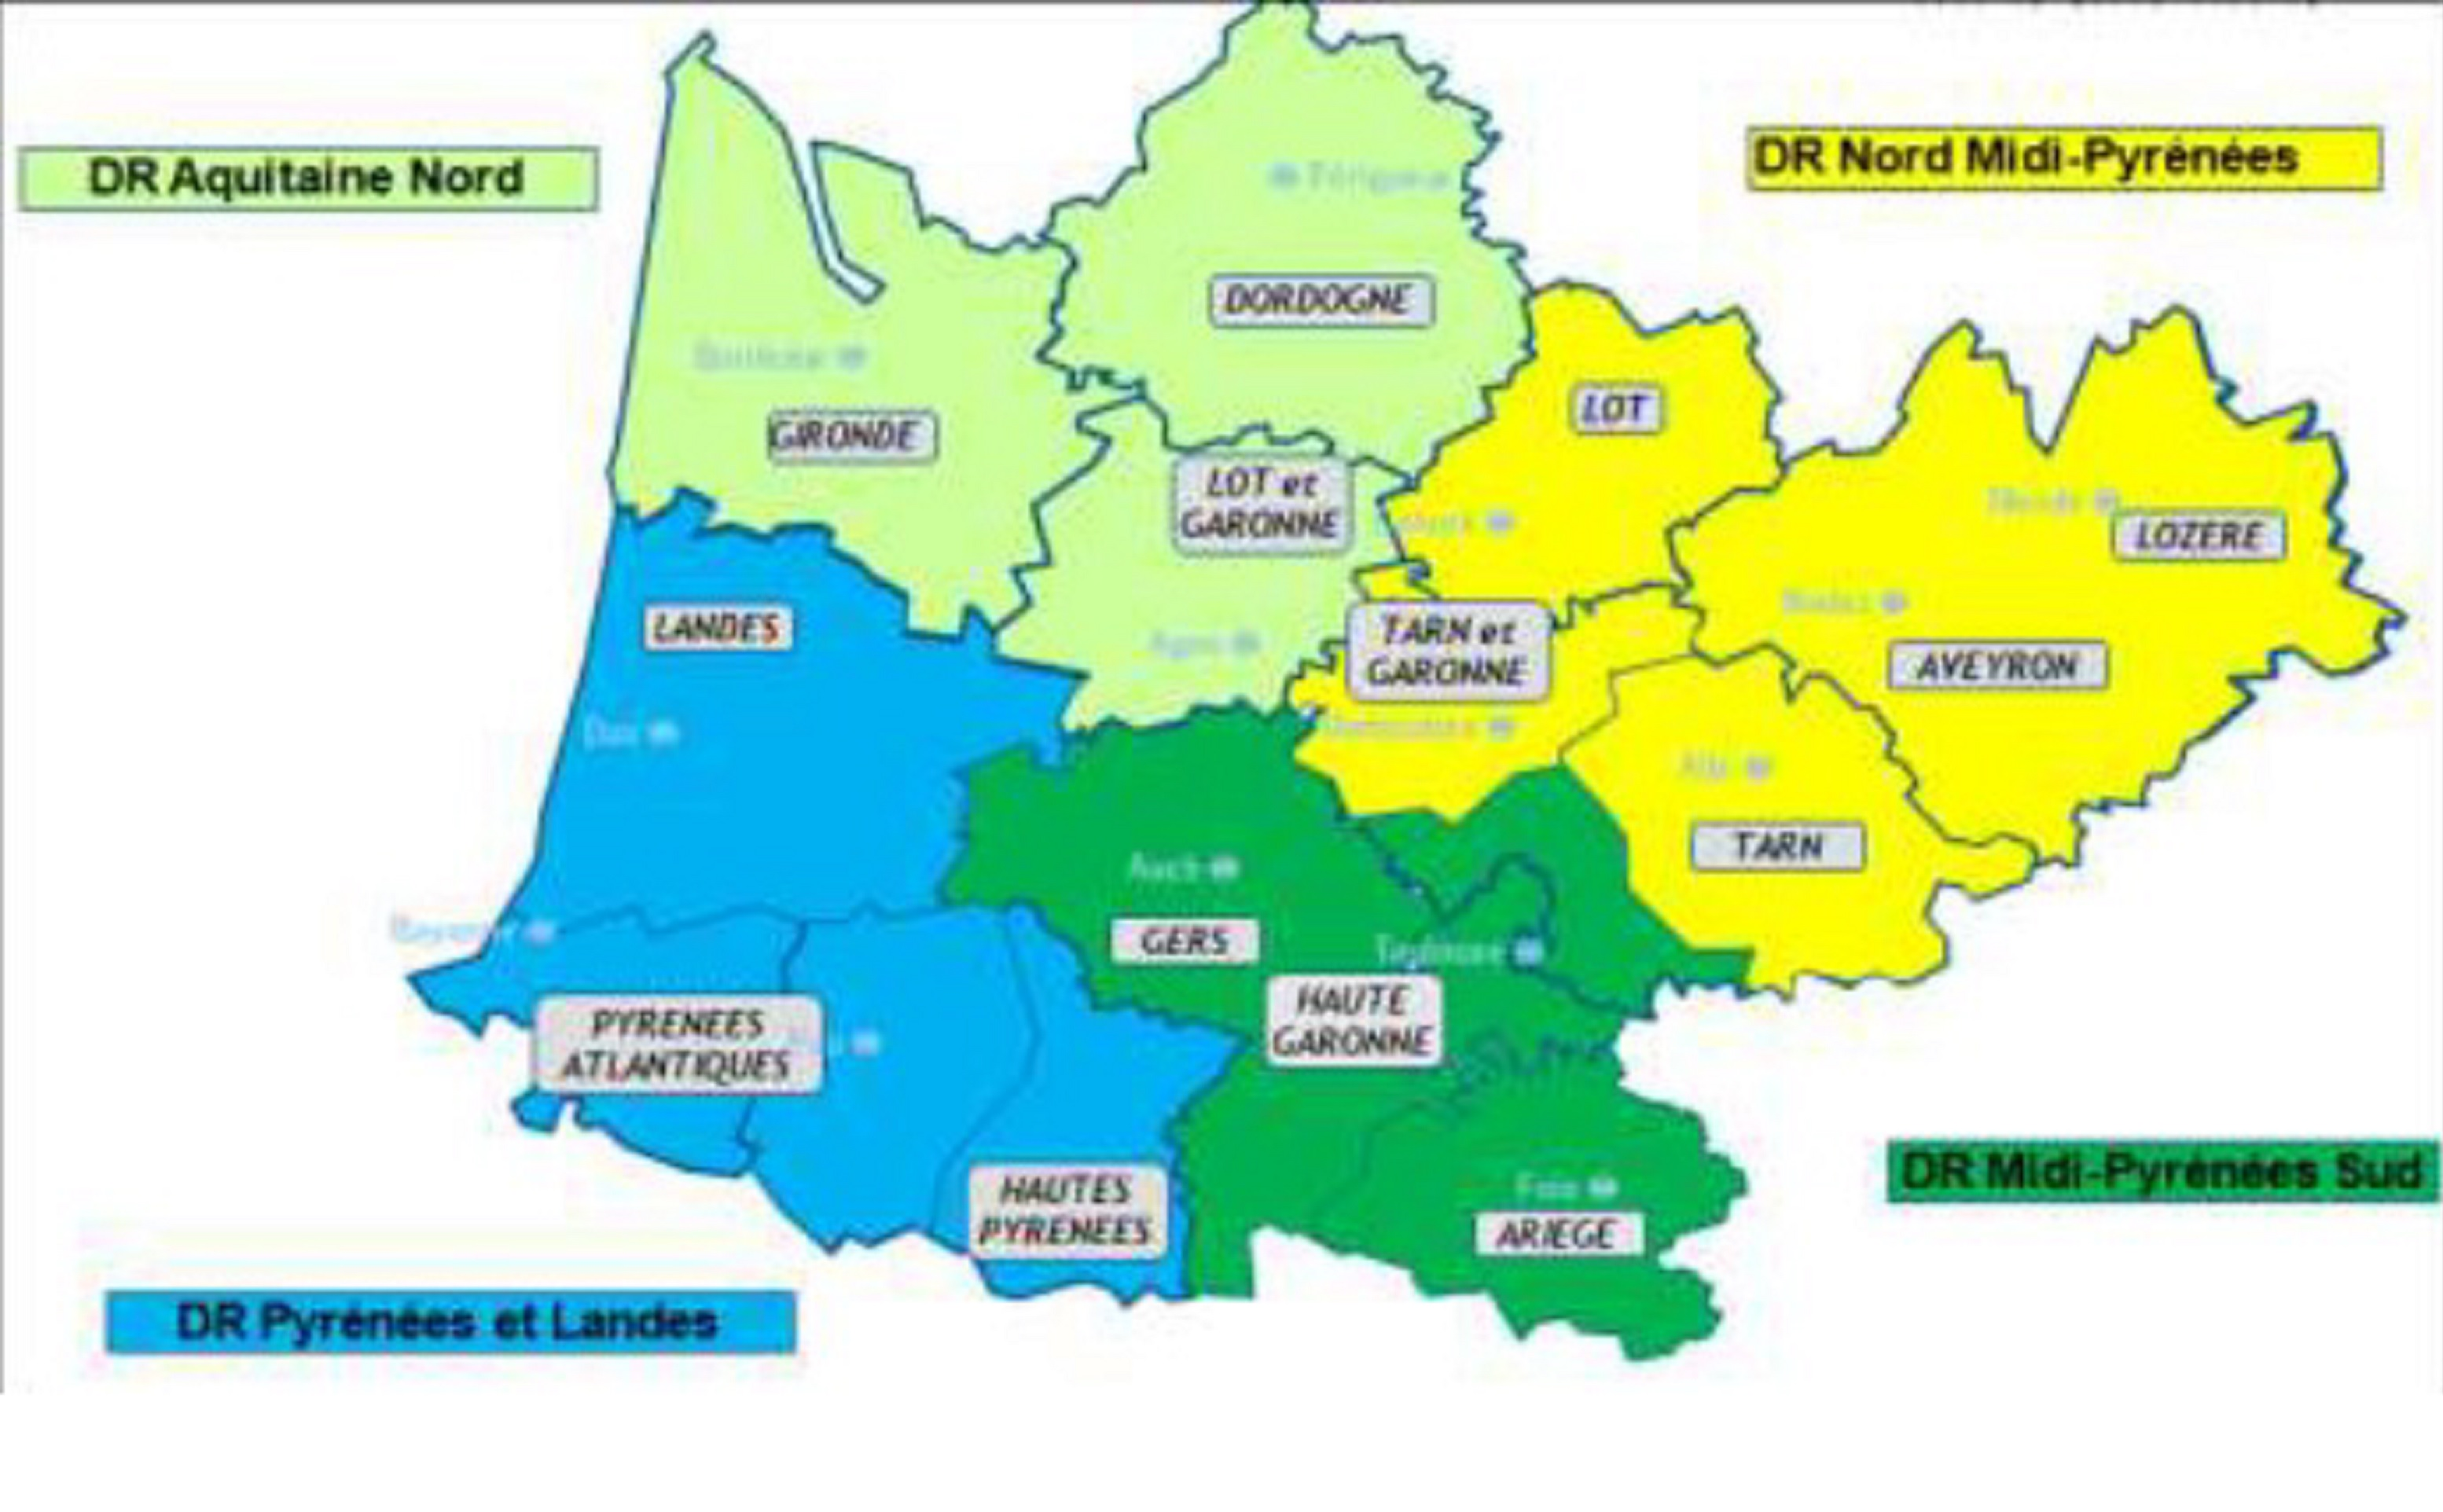
\includegraphics[width=13cm]{dir.jpg}
\caption{\label{dirso}la répartition des 4 DR à la maille Sud Ouest}
\end{figure}
Le rôle des DR est de construire un projet stratégique de région, d'être responsable de la vie des concessions et de la conduite des opérations et de piloter sa performance financière, sociale, technique et patrimoniale.

\subsection*{Direction Technique}
 Elle a été créée pour répondre aux enjeux d'ERDF en inter-région Sud Ouest et pour s'adapter aux évolutions de l'environnement externe et interne.
Elle a aussi un enjeu financier à travers les prévisions budgétaires annuelles attribuées pour chaque Direction Régionale.
Cette Direction Technique présidée par Thierry MARTINEZ, a un champ d'action dans toutes les DR et
dispose de 3 sites basés à TOULOUSE (31), BORDEAUX (33) et AGEN (47).
Son rôle est de préparer et porter les politiques techniques, d'animer les 3 domaines métiers en inter-région (patrimoine – réseau – Poste Source), d'assurer les études électriques en co-construction avec les DR.
Pour exercer ses différentes missions, la Direction Technique est organisée en 7 pôles d'activités
qui sont:
\begin{itemize}
\item Pôle Études et Maîtrise Ouvrage HTA
\item Pôle Maîtrise Ouvrage Postes Sources
\item Pôle Grand Producteur\footnote{Pendant mon stage de l'année dernière (2013-2014), j'ai développé un outil de suivi et de pilotage d'activité pour ce pôle}
\item Expertise Technique et SI
\item Économie Concessionnaire
\item Politique Industrielle
\item Politique Programme Performance
\end{itemize}
Je me situe quant à moi dans le \og Pôle Études et Maîtrise Ouvrage HTA\fg{} que je vais vous présenter.\\ Le pôle \og Études et Maîtrise d'ouvrage HTA\fg{} est constitué de 3 métiers, comme le montre le schéma~\ref{metier} ci-dessous:
\begin{figure}[h]
\centering
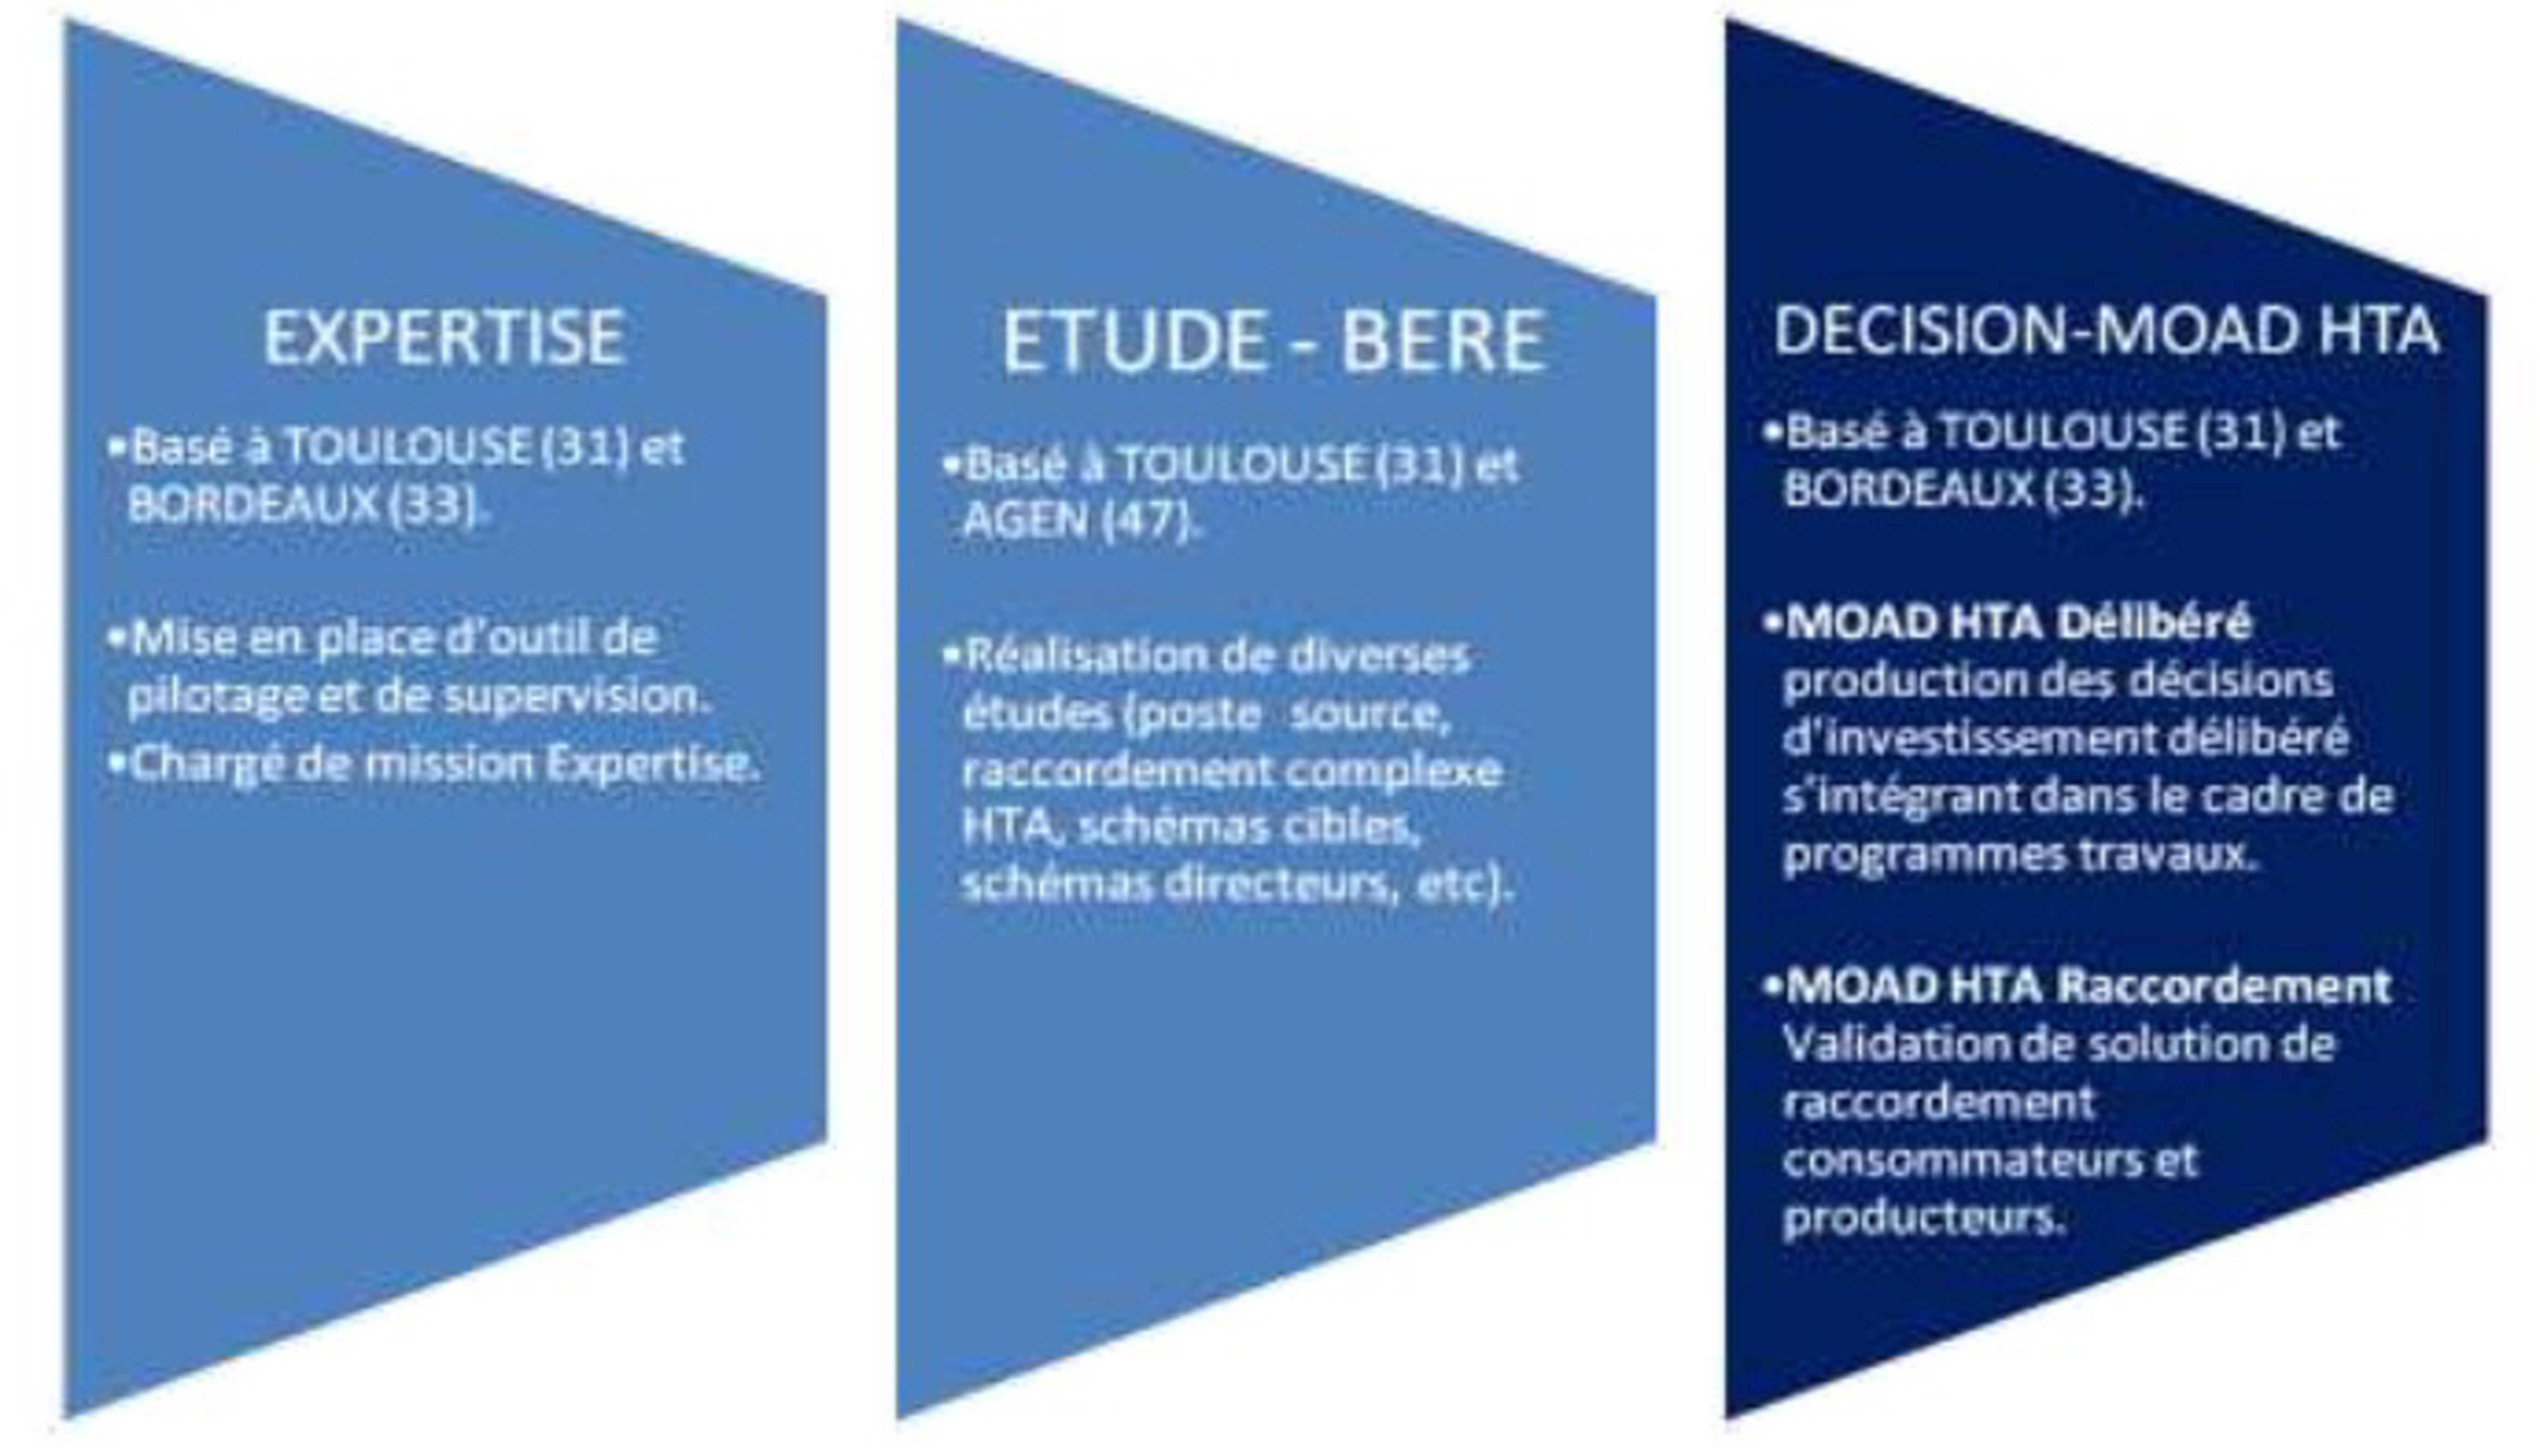
\includegraphics[width=13cm]{metier.jpg}
\caption{\label{metier}les métiers du pôle \og Études et Maîtrise d’ouvrage HTA\fg{}}
\end{figure}
Le but de ma mission est donc de créer un portail de travail collaboratif afin que les BERE ainsi que la maitrise d'ouvrage pour qu'il puisse travailler ensemble afin d'améliorer leurs résultats. 
